\section{La planification}

\frame{
\frametitle{Techniques de planification}
\begin{center}
Objectif : gérer le découpage temporel et structurel
\end{center}
\vspace{.8cm}

\underline{Techniques} :
\vspace{.5cm}
\begin{itemize}
\item Graphe PERT pour :
	\begin{itemize}
	\item mettre en évidence les dépendances entre tâches
	\item mettre en évidence le parallélisme potentiel
	\item calculer la durée minimum du projet
	\item mettre en évidence les temps d'attente
	\end{itemize}
	\vspace{.3cm}
\item Diagramme Gantt pour :
	 \begin{itemize}
	 \item faire des hypothèses sur les \emph{ressources}
	 \item faire des hypothèses sur les disponibilités
	\item  établir un calendrier de travail
	\end{itemize}
\end{itemize}
\vspace{1cm}	
 
}
%*****************************************************************
\subsection{Méthode PERT}
\frame{
\frametitle{Méthode PERT}
\begin{center}
Project Evaluation and Review Technique (PERT)
\end{center}
\vspace{.3cm}

\begin{itemize}
\item \'{E}tablissement de l'ensemble des tâches et leurs durée estimée
\item Ordonnancement des tâches selon dépendances
\end{itemize}
 
 \input pert.pdftex_t
  
\vfill 
}
%*****************************************************************
\frame{
\frametitle{Méthode PERT (2)}

%% Graphes utilisés pour représenter les dépendances

\noindent \input pert2.pdftex_t
}
%*****************************************************************
\frame{
\frametitle{Graphe PERT}

\begin{itemize}
\item Le projet est caractérisé par 
\begin{itemize}
	\item	un ensemble de tâches $T$
	\item	une date de début $t_0$
	\item	une date de fin	$t_f$
\end{itemize}
\vspace{3mm}
\item Une tâche $T_i$ possède :
\begin{itemize}
	\item une durée $d({T_i})$
	\item un ensemble de prédécesseurs $Pred(T_i)$
	\item un ensemble de successeurs $Succ(T_i)$
\end{itemize}
\end{itemize}

$\Rightarrow$ Objectif : définir  

\begin{itemize}
	\item la date \emph{au plus tôt} de chaque tâche  
	\item la date \emph{au plus tard} de chaque tâche
	\item le \emph{chemin critique}
\end{itemize}

}
%*****************************************************************
\frame{
\frametitle{Dates au plus tôt}

\begin{tabular}{ll}

	 la tâche ne peut débuter avant & $d_{tot}(T_i)$ 	\\
	 la tâche ne peut finir avant	& $f_{tot}(T_i)$  	\\

\end{tabular} 

$$\begin{array}{|ll|}
\hline
d_{tot}(T_i) = &
	 \left\{\begin{array}{ll}
		 max(f_{tot}(Pred(T_i)))& {\rm si}~ Pred(T_i) \not= \{\}\\
		 t_0			& {\rm sinon} \\
	\end{array}\right. \\	 
f_{tot}(T_i) = & d_{tot}(T_i) + d(T_i)\\
\hline
\end{array}^{\star}$$
 
\vspace{1cm}
$\star$ : si tous les liens sont de type fin-début
}
%*****************************************************************
\frame{
\frametitle{Dates au plus tard}

\begin{tabular}{ll}

	 la tâche doit débuter au plus tard à & $d_{tard}(T_i)$ 	\\
	 la tâche doit finir au plus tard à	& $f_{tard}(T_i)$  	\\

\end{tabular} 

$$\begin{array}{|ll|}
\hline
f_{tard}(T_i) = &
	 \left\{\begin{array}{ll}
		 min(d_{tard}(Succ(T_i)))& {\rm si}~ Succ(T_i) \not= \{\}\\
		 t_f			& {\rm sinon} \\
	\end{array}\right. \\	 
d_{tard}(T_i) = & f_{tard}(T_i) - d(T_i)\\
\hline
\end{array}^{\star}$$


\vspace{1cm}
$\star$ : si tous les liens sont de type fin-début
}
%************************************************************************
\frame{
\frametitle{Exemple dates au plus tôt}
 
\input pert3.pdftex_t
 
\vspace{1cm}
Remarquer la tâche $T_5$ avec plusieurs prédécesseurs :

$$d_{tot}(T_5) = max(\{f_{tot}(T_2);f_{tot}(T_3)\})) = max(\{7,10\})=10$$
}
%************************************************************************
\frame{
\frametitle{Exemple dates au plus tard}

Supposons $t_f = 15$ (estimation de la fin du projet)  
 
\vspace{1cm}
 
\input pert4.pdftex_t
 
 
}
%************************************************************************
\frame{
\frametitle{Marges et chemin critique}

\begin{itemize}
\item[$\bullet$]
	Marge (de man\oe uvre) : 
	$ \begin{array}[t]{ll} 
		m(T_i) & = d_{tard}(T_i) - d_{tot}(T_i) \\
		  & = f_{tard}(T_i) - f_{tot}(T_i)  
	\end{array}$
	\item[$\bullet$] Chemin critique : \\
	chemin tel que la somme des marges est minimale
	
	\item[$\bullet$] Cas particulier avec uniquement liens fin-début\\
	Chemin critique $\Leftrightarrow$ Chemin le plus long
	
 \end{itemize}
\vspace{.3cm}
 
\input pert5.pdftex_t
 
Ici : le chemin critique est $\{T_1;T_3;T_5\}$  
}
%************************************************************************
\frame{
\frametitle{Exercice graphe PERT}

\begin{tiny}
\[\begin{tabular}{|l|l|l|}
\hline\hline
Tâche		& durée	& lien	\\
\hline
$t_1$		& 5	& fin $t_1$ - début $t_3$ \\ \hline
$t_2$		& 2	& fin $t_2$ - début $t_4,t_5$ \\ \hline
$t_3$		& 10	& fin $t_3$ - début $t_6,t_8$ \\ \hline
$t_4$		& 8	& fin $t_4$ - début $t_6$ \\ \hline
$t_5$		& 10	& fin $t_5$ - début $t_7$ \\ \hline
$t_6$		& 25	& fin $t_6$ - début $t_{11}$ \\ \hline
$t_7$		& 4	& fin $t_7$ - début $t_{11}$ \\ \hline
$t_8$		& 10	& fin $t_8$ - début $t_9,t_{10},t_{11}$ \\ \hline
$t_9$		& 2	& fin $t_9$ - début $t_{13}$ \\ \hline
$t_{10}$	& 1	& fin $t_{10}$ - début $t_{13}$ \\ \hline
$t_{11}$	& 15	& début $t_{11}$ - début $t_{12}$ \\ 
		&	& fin $t_{11}$ - début $t_{13}$ \\ \hline	
$t_{12}$	& 10	& fin $t_{12}$ - début $t_{14}$ \\ \hline
$t_{13}$	& 12	& fin $t_{13}$ - fin  \\ \hline
$t_{14}$	& 30	& fin $t_{14}$ - fin \\
\hline
\end{tabular}\]
\end{tiny}
}
%************************************************************************
\subsection{Méthode PERT probabiliste}
\frame{
\frametitle{PERT Probabiliste: synopsis}

\begin{itemize}
\item<+-> Inclure risque et incertitude dans la durée

\item<+-> Durée d'une tâche considérée comme une variable aléatoire
(dont la distribution suit une loi Beta).

\item<+-> 
\begin{tabular}[t]{p{.6\textwidth}c}
La durée totale est aussi une variable aléatoire suivant une loi normale (théorème de la limite centrale).&
\end{tabular}
%--------- comment -------------
%théorème de la limite centrale: la somme de variables aléatoires indépendantes est une variable aléatoire suivant une loi normale). 
% En se positionnant en univers certain et en utilisant les durées moyennes
% obtenues avec la loi Beta. 


\item<+-> Conditions
\begin{itemize}
	\item nombre suffisant de tâches
	\item ordre de grandeur semblables pour les durées
	\item indépendances entre durées des tâches
\end{itemize}
\end{itemize}
\pgfputat{\pgfxy(8,1)}{\pgfbox[left,base]{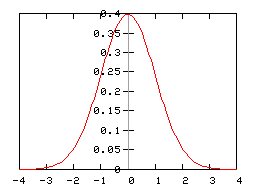
\includegraphics[width=4cm]{gaussreduite.png}}}
}

%************************ Pourqoui Beta ? *********************************
\frame{
\frametitle{Loi pour la durée d'une tâche}

Une loi adéquate est la distribution \textbf{Beta}.
\pause

\begin{center}
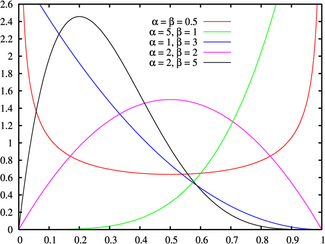
\includegraphics[height=.5\textheight]{betapdf_general.png}
\end{center}

\begin{itemize}
\item<+-> On peut contrôler la forme de la courbe avec $\alpha$ et $\beta$.
\item<+-> En particulier, elle peut être asymétrique (e.g. allongée à droite).
\item<+-> Elle a des limites finies (comme les durées de tâches).
\end{itemize}
}
%************************************************************************
\frame{
\frametitle{Loi pour la durée d'une tâche}

\uncover<1>{Fonction de densité de la distribution:
$$ f(x)=\frac{(x-a)^{p-1}(b-x)^{q-1}}{(b-a)^{p+q-1}B(p,q)} ~~~ a \leq x \leq b ; p,q > 0$$
  	 avec $B$ la fonction beta:
  	 $ B(p,q)=\int_0^1 t^{\alpha-1}(1-t)^{\beta-1} dt$

\vspace{1cm}
}
\pause

Les travaux de C. Clarke (1962) ont donné une méthode pour contrôler
$\alpha$ et $\beta$ à partir de 3 paramètres plus simples : \\
\pause

\begin{tabular}[t]{ll}
	$opt$ : & durée optimiste\\
	$pes$ : &  durée pessimiste\\
	$vrai$ : & durée vraisemblable\\
\end{tabular}

% $$ f(x)=\frac{(x-a)^{p-1}(b-x)^{q-1}}{(b-a)^(p+q-1)B(p,q)} ~~~ 0 \leq x \leq 1 ; p,q > 0$$
%  	 avec $B$ la fonction beta:
%  	 $ B(p,q)=\int_0^1 t^{\alpha-1}(1-t)^{\beta-1} dt$
  	
%
% p = 3 + sqrt{2}    q = 3 - sqrt{2}   si m > (a+b)/2
% p = 3 - sqrt{2}    q = 3 + sqrt{2}   si m > (a+b)/2

}
%************************************************************************
\frame{
\frametitle{PERT probabiliste (2)}
 

Pour une tâche :
\begin{itemize}
\item
Calculer la durée probable d'une tâche $i$ : 
\[
	prob_i = \frac{opt_i + 4~vrai_i + pes_i}{6}
\]
 

\item Mesurer l'incertitude de l'estimation en \\
calculant l'indicateur de dispersion de la durée de la tâche $i$:

\[ d_i = \frac{pes_i - opt_i}{6} \]

\end{itemize}
}
%************************************************************************
\frame{
\frametitle {PERT probabiliste (3)}
Pour un chemin constitué des tâches $\{1;2; ...;n\}$ \\
\begin{itemize}
\item Mesurer la durée estimée du chemin 
\[	D = \sum_{i=1}^n prob_i \]

\item Mesurer l'écart-type de l'estimation pour le chemin :
\[ E = \sqrt{\sum_{i=1}^n d_i^2} \]
\end{itemize}
}
\begin{comment}
Note sur la variance et l'écart-type :
Exemple : on a $k$ notes $\{n_1, ..., n_k\}$. La moyenne est
$m=(\sum_{i=1}^k n_i) /k$.
La variance est $v = (\sum_{i=1}^k (n_i-m)^2)/k$ et l'écart-type
est $\sigma=\sqrt{v}$.
\end{comment}
%************************************************************************
\frame{
\frametitle{PERT probabiliste (4)}

	Obtenir la durée du chemin avec une probabilité $p$ :
	\[ {\cal D}(p) = D + E \times G(p) \] 

où $G$ est la fonction associée à la loi normale centrée réduite (extrait)  :

\[\begin{tabular}{|l|l||l|l|}
\hline
$p$	&	$G(p)$	&$p$		&	$G(p)$ \\
\hline
99,9	& 	3,00    & 89,1		& 	1,23	\\ 
99	& 	2,31	& 85,1		&	1,04	\\
98	& 	2,06	& 70,2		& 	0,53	\\
97	&	1,88	& 50		&	0	\\
95	& 	1,65	& 42,1		& 	-0,2	\\
92,1	&	1,41	& 34,5		& 	-0,4	\\
90	&	1,28	& 27,4		&	-0,6	\\ 		
\hline	
\end{tabular}\]

}
%************************************************************************
\frame{
\frametitle{PERT probabiliste (4)}
\underline{Exemple} : Les estimations sont $D = 100$ et  $E = 15$.\\

	La durée probable à 90\% est
	$$\begin{array}[t]{ll} 
	  {\cal D}(90)	& = 100 + 15 \times G(90) \\
	  		& = 100 + 15 \times 1,28\\
			& \approx 119\\
	\end{array}$$ 


	La durée probable à 70\% est
	$$\begin{array}[t]{ll} 
	  {\cal D}(70)	& = 100 + 15 \times G(70) \\
	  		& = 100 + 15 \times 0,53\\
			& \approx 108\\
	\end{array}$$ 
	
	La probabilité de terminer en 90 jours est
	$$\begin{array}[t]{ll} 
	  90	& = 100 + 15 \times G(p) \\
	  G(p)	& = -10 / 15 = -2 / 3\\
	 \end{array}$$
	d'où ~~~$ p \approx 27\% $ 
}
%************************************************************************
\frame
{\frametitle
{Exercice PERT probabiliste}

\begin{tabular}{|l|l|l|l|l|}
\hline 
$t_i$	& Description	& {\small $opt$}	&  {\small $pes$} & {\small
$vrai$} \\
\hline
$t_1$ & {\small faire fondre le beurre et le chocolat}	& 6	& 9	& 7,5	\\
$t_2$ & {\small séparer les oeufs en jaunes et blancs}	& 1	& 4,5	& 3	\\
$t_3$ & {\small ajouter les jaunes au mélange, faire cuire} & 6 & 8 & 7	\\
$t_4$ & {\small monter les blancs en neige}	& 2 	& 12 	& 5	\\
$t_5$ &	{\small arrêter la cuisson du mélange,}	&	& & \\
      & {\small et incorporer les blancs au mélange}	& 2 & 6 & 3\\
$t_6$ & {\small faire cuire au four}	& 16 & 22 & 18\\
\hline
\end{tabular}

\textit{\small 
\begin{enumerate}
\item Tracer le graphe PERT (sans contrainte de ressources)
\item Calculer la durée probable, l'écart-type de chaque chemin
\item Déterminer le chemin critique
\item Quelle est la durée estimée de préparation du gâteau,
	\begin{itemize}
	\item[--] avec une probabilité de 90\% ?
	\item[--] avec une probabilité de 95\% ?
	\end{itemize}
\item Quelle est la probabilité de terminer en 37 minutes ?	
\end{enumerate}
}
}
%************************************************************************
%* Corrigé
%*
\begin{comment}
      prob   d_i    d_i^2
T1    7.5    1/2    1/4
T2    2.91   0.58   0.34
T3    7      1/3    2/9
T4    5.66   5/3    25/9
T5    3.33   2/3    4/9
T6    18.33  1      1

Examinons les différents chemins :
        +-- T1 --> T3 --+
        |         ^     |
debut --+        /      +--> T5 --> T6 --> fin
        |      /        |
        +-- T2 --> T4 --+
$$
C_1 = \{ T2;T3;T5;T6\}
C_2 = \{ T1;T3;T5;T6\}
C_3 = \{ T2;T4;T5;T6\}

D_{C_1} = 31.57   E_{C_1} = 1.38
D_{C_2} = 36.16   E_{C_2} = 1.34
D_{C_3} = 30.23   E_{C_3} = 2.14

Durée probable avec fiabilité à 90\% , à 95\%
==============================================
{\cal D}(0.9) = D_{C_2} + E_{C_2} * G(0.9)
              = 37.87 (37 min 52 s)
{\cal D}(0.95) = 38,38
=> relativement peu d'incertitude

Comparaison des chemins
=======================
      0.95   0.9
C_1   33.86  33.35
C_2   38.38  37.89
C_3   33.77  32.98

Probabilité x de terminer en 37 min ou moins
============================================
On prend le plus long dans presque (?) tous les cas : C_2
on a :
   {\cal D}(x) = D_{C_2} + G(x).E_{C_2} 
            37 = 36.16 + G(x). 1.34
            G(x) = 0.619
       <=>  x = 72\%

A partir de quelle probabilité x a t-on {\cal D}_{C_3}(x) > {\cal D}_{C_2}(x) ?
==============================================================================
        33.77 + G(x)*2.14    > 36.16 + G(x)* 1.34
        G(x) > 2.98

$$
\end{comment}


%************************************************************************
\subsection{Diagramme Gantt}
\frame{
\frametitle{Diagramme Gantt}
\vspace{.2cm}
\begin{center}
	Etablir un planning
\end{center}
\vspace{.3cm}

\begin{itemize}
\item<+-> Un réseau PERT donne les dates (au plus tôt, au plus tard) sans tenir compte des contraintes de ressources\\
\item<+-> Planning $\Rightarrow$ faire des hypothèses sur les ressources\\
\item<+-> Diagramme Gantt : qui fait quoi et quand ?\\

\item<+-> Possibilité de modifier le planning en 
	\begin{itemize}
	\item jouant sur les ressources affectées
	\item jouant sur le chargement (au plus tôt, au plus tard)
	\end{itemize}
\end{itemize}

}
%************************************************************************
\frame{
\frametitle{Diagramme Gantt (2)}

\input{pert5.pdftex_t}

\underline{Hypothèses} : ressources R1 et R2, et chargement au plus tôt\\
\pause

\input{gantt1.pdftex_t} 

}
%************************************************************************
\frame{
\frametitle {Diagramme de Gantt (3)}

\input{pert5.pdftex_t}

\underline{Hypothèses} : ressources R1 et R2, et chargement au plus tard\\
\pause

\input{gantt2.pdftex_t} 
\vfill
}
%************************************************************************
\frame{
\frametitle{Diagramme Gantt : le nivellement}
\vspace{.4cm}
Le \emph{nivellement} : limiter les ressources utilisées 
 
\vspace{.8cm} 
\begin{center}
\input{gantt4.pdftex_t} 
\end{center}

}
%************************************************************************
\frame{
\frametitle{Diagramme Gantt : le lissage}

\vspace{.3cm}

Le \emph{lissage} : répartir l'utilisation d'une ressource dans le temps

\vspace{.3cm}

\begin{center}
\input{gantt3.pdftex_t} 
\end{center}
}



